%%%%%%%%%%%%%%%%%%%%%%%%%%%%%%%%%%%%%%%%%
% Beamer Presentation
% LaTeX Template
% Version 1.0 (10/11/12)
%
% This template has been downloaded from:
% http://www.LaTeXTemplates.com
%
% License:
% CC BY-NC-SA 3.0 (http://creativecommons.org/licenses/by-nc-sa/3.0/)
%
%%%%%%%%%%%%%%%%%%%%%%%%%%%%%%%%%%%%%%%%%

%----------------------------------------------------------------------------------------
%	PACKAGES AND THEMES
%----------------------------------------------------------------------------------------

\documentclass{beamer}

\mode<presentation> {

% The Beamer class comes with a number of default slide themes
% which change the colors and layouts of slides. Below this is a list
% of all the themes, uncomment each in turn to see what they look like.

%\usetheme{default}
%\usetheme{AnnArbor}
%\usetheme{Antibes}
%\usetheme{Bergen}
%\usetheme{Berkeley}
%\usetheme{Berlin}
%\usetheme{Boadilla}
\usetheme{CambridgeUS}
%\usetheme{Copenhagen}
%\usetheme{Darmstadt}
%\usetheme{Dresden}
%\usetheme{Frankfurt}
%\usetheme{Goettingen}
%\usetheme{Hannover}
%\usetheme{Ilmenau}
%\usetheme{JuanLesPins}
%\usetheme{Luebeck}
%\usetheme{Madrid}
%\usetheme{Malmoe}
%\usetheme{Marburg}
%\usetheme{Montpellier}
%\usetheme{PaloAlto}
%\usetheme{Pittsburgh}
%\usetheme{Rochester}
%\usetheme{Singapore}
%\usetheme{Szeged}
%\usetheme{Warsaw}

% As well as themes, the Beamer class has a number of color themes
% for any slide theme. Uncomment each of these in turn to see how it
% changes the colors of your current slide theme.

%\usecolortheme{albatross}
%\usecolortheme{beaver}
%\usecolortheme{beetle}
%\usecolortheme{crane}
%\usecolortheme{dolphin}
%\usecolortheme{dove}
%\usecolortheme{fly}
%\usecolortheme{lily}
%\usecolortheme{orchid}
%\usecolortheme{rose}
%\usecolortheme{seagull}
%\usecolortheme{seahorse}
%\usecolortheme{whale}
%\usecolortheme{wolverine}

%\setbeamertemplate{footline} % To remove the footer line in all slides uncomment this line
%\setbeamertemplate{footline}[page number] % To replace the footer line in all slides with a simple slide count uncomment this line

%\setbeamertemplate{navigation symbols}{} % To remove the navigation symbols from the bottom of all slides uncomment this line
}

\usepackage[orientation=landscape,size=custom,width=16,height=9,scale=0.4]{beamerposter}
\usepackage[utf8x]{inputenc}
\usepackage{algorithmicx}
\usepackage{algorithm}% http://ctan.org/pkg/algorithms
\usepackage{algpseudocode}% http://ctan.org/pkg/algorithmicx
\usepackage{amsfonts}
\usepackage{amsmath,amssymb,amstext,mathabx}
\usepackage{amsmath}
\usepackage{amsthm,lipsum}
\usepackage{booktabs} % Allows the use of \toprule, \midrule and \bottomrule in tables
\usepackage{graphicx} % Allows including images
\usepackage{hyperref}
\usepackage{listings}
\usepackage{subcaption}
\setbeamersize{text margin left=5em}  % <- like this
\setbeamersize{text margin right=5em} % <- like this

%My Maths operators
\DeclareMathOperator{\opt}{opt}
\DeclareMathOperator{\web}{web}
\DeclareMathOperator{\PO}{PO}
\DeclareMathOperator{\DM}{DM}
\DeclareMathOperator{\MT}{MT}
\DeclareMathOperator{\mtx}{mtx}
\DeclareMathOperator{\nrows}{nrows}
\DeclareMathOperator{\ncols}{ncols}
\DeclareMathOperator{\potpos}{Potential Positions}
\DeclareMathOperator{\nodf}{nodf}
\DeclareMathOperator{\NODF}{NODF}
\DeclareMathOperator{\neighbor}{neighbor}
\DeclareMathOperator{\random}{random}
\DeclareMathOperator{\cost}{cost}
\DeclareMathOperator{\hillclimb}{Hillclimb}
\DeclareMathOperator{\Olap}{O}
\DeclareMathOperator{\DF}{DF}
\DeclareMathOperator{\row}{row}
\DeclareMathOperator{\col}{col}
\DeclareMathOperator{\Fmin}{Fmin}
\newcommand{\N}{\mathbb{N}}
\newcommand{\R}{\mathbb{R}}

\setbeamertemplate{navigation symbols}{}
\beamertemplatenavigationsymbolsempty

%\newenvironment{sysmatrix}[1]
% {\left(\begin{array}{@{}#1@{}}}
% {\end{array}\right)}
%\newcommand{\ro}[1]{%
%  \xrightarrow{\mathmakebox[\rowidth]{#1}}%
%}
%\newlength{\rowidth}% row operation width
%\AtBeginDocument{\setlength{\rowidth}{3em}}

%----------------------------------------------------------------------------------------
%	TITLE PAGE
%----------------------------------------------------------------------------------------

\title[T-Shirt Problem]{Optimising T-Shirt distributiuon} % The short title appears at the bottom of every slide, the full title is only on the title page

\author{A. Puiu, Y. Tian, J. Dyer, C. Hoeppke} % Your name
\institute[University of Oxford] % Your institution as it will appear on the bottom of every slide, may be shorthand to save space
{
%University of Oxford\\
%\medskip
\textit{Department for Mathematics} % Your email address
\date{\today} % Date, can be changed to a custom date
}
%\date{01/10/2018} % Date, can be changed to a custom date
\begin{document}


\begin{frame}
%Probably the titlepage will not be needed!
\titlepage % Print the title page as the first slide
\end{frame}

% Christophe
\section{Description of the Problem}
% Describe the problem
% Problem description section


% Joel
\subsection{Brute force approach}
% Use this the clarify why the problem is difficult.
% Put bruteforce section here
\begin{frame}
Brute force approach:
\begin{lstlisting}[language=Python]
for each number N of box types:
	for each combination of N distinct box types:
		calculate penalty given N and the over- and under-stock
\end{lstlisting}
However, there are $\sim 10^{11}$ boxes possible, so $\sim 2^{10^{11}} - 1$ penalties to calculate $\Rightarrow$ brute force unfeasible
\end{frame}



\section{Pattern detection}
% Section that contains the pattern detection
\begin{frame}{Initial Analysis}
	The Data:
	\begin{itemize}
		\item 58 stodes with 4 colours and 6 sizes each.
		\item only M and L for black, blue and red can be overstacked.
	\end{itemize}
	Fundamental Problem:
	\begin{itemize}
		\item Boxes require even number of shirt, but some stores order odd numbers $\Rightarrow$ overstocking is unavoidable.
	\end{itemize}
	Try to find further structure:
	\begin{itemize}
		\item min,average,mode,sum $Rightarrow$ subtract the mode $Rightarrow$ subtract the min $\Rightarrow$ pattern inside each colour
	\end{itemize}
\end{frame}
\begin{frame}{Initial Analysis ct'd}

\begin{equation}
    \begin{bmatrix}
    1&2&2&3&2&1\\
    0&0&2&0&0&0\\
    0&0&0&2&0&0\\
    0&0&0&0&2&0
    \end{bmatrix}
\end{equation}
\begin{equation}
\color{blue}
    \begin{bmatrix}
        1&2&2&3&3&1\\
        0&0&0&2&0&0\\
        0&0&1&0&1&0\\
        0&0&1&1&0&0\\
    \end{bmatrix}
\end{equation}
\begin{equation}
\color{red}
    \begin{bmatrix}
         1&2&3&3&3&1\\
         0&0&0&1&2&0\\
         0&0&0&3&0&0\\
         0&1&1&0&0&0\\
    \end{bmatrix}
\end{equation}
\begin{equation}
\color{green}
    \begin{bmatrix}
         0&0&0&0&0&0\\
         1&1&1&2&1&1\\
         1&1&2&2&1&1\\
         1&1&2&2&2&1\\
    \end{bmatrix}
\end{equation}
\end{frame}

\begin{frame}{Colour Based Optimisation}
	\begin{itemize}
		\item We form boxes for each colour individually
	\end{itemize}
	\begin{equation*}
     \begin{bmatrix}
     1&2&2&3&2&1\\
  0&0&2&0&0&0\\
  0&0&0&2&0&0\\
  0&0&0&0&2&0
         \end{bmatrix} \Rightarrow
     \begin{bmatrix}
     1&2&2&2&2&1\\
	     0&0&2&1+\Color{Red}1&0&0\\
	     0&0&0&3+\Color{Red}1&0&0\\
	     0&0&0&1+\Color{Red}1&2&0
     \end{bmatrix}
	\end{equation*}
	\begin{equation*}
    \color{blue}
    \begin{bmatrix}
        1&2&2&3&3&1\\
        0&0&0&2&0&0\\
        0&0&1&0&1&0\\
        0&0&1&1&0&0\\
    \end{bmatrix}\Rightarrow
    \color{blue}
    \begin{bmatrix}
        1&2&2&2&2&1\\
        0&0&0&3&1&0\\
        0&0&1&1&2&0\\
        0&0&1&2&1&0\\
    \end{bmatrix}
	\end{equation*}
\end{frame}
\begin{frame}
	\begin{equation}
	\color{red}
    \begin{bmatrix}
         1&2&3&3&3&1\\
         0&0&0&1&2&0\\
         0&0&0&3&0&0\\
         0&1&1&0&0&0\\
    \end{bmatrix}\Rightarrow \begin{bmatrix}
	    1&2&2&2&2&1\\
         0&0&1&2&3&0\\
         0&0&1&4&1&0\\
	    0&1&2&1&1+\Color{Grey}1&0\\
    \end{bmatrix}
\end{equation}
\begin{equation}
\color{green}
    \begin{bmatrix}
         0&0&0&0&0&0\\
         1&1&1&2&1&1\\
         1&1&2&2&1&1\\
         1&1&2&2&2&1\\
    \end{bmatrix}\Rightarrow
    \begin{bmatrix}
         1&1&1&2&1&1\\
         1&1&2&2&1&1\\
         1&1&2&2&2&1\\
    \end{bmatrix}
\end{equation}
$\Rightarrow$ This gives $4+5+4+3=16$ types, but we can do better for blue!

\begin{frame}
\begin{equation}
    \begin{bmatrix}
        1&2&2&2&2&1\\
        0&0&0&3&1&0\\
        0&0&1&1&2&0\\
        0&0&1&2&1&0\\
    \end{bmatrix} \Rightarrow \begin{bmatrix}
	    1& 0& 0& 1& 3& 1\\
	    0& 1& 2& 1& 0& 0\\
	    0& 1& 1& 2& 0& 0\\
	    0& 1& 1& 1& 1& 0 \\
    \end{bmatrix}
	\end{equation}
    $\Rightarrow$ Now $16-1=15$ types.
\end{frame}
\begin{frame}{Cross Colour Optimisation}
	\begin{itemize}
	\item full rank now, to further reduce the types of boxes, we need to consider the combination of them
	\item to avoid the mess of combination for each store, we consider combine the box 1 in black and box 1 in blue, as they are what everybody needs
	\end{itemize}
    \begin{equation}
        \begin{bmatrix}
            0& 0& 0& 0& 2& 1\\
            1& 2& 4& 3& 0& 0 \\
             1& 2& 2& 5& 0& 0\\
             1& 2& 2& 3& 2& 0
        \end{bmatrix}
    \end{equation}
			$\Rightarrow$ then combine the box 1 in black with box 1 in blue with extra 1 in black L (acceptable overload)
now $15 – 1 = 14$ types!
	\end{frame}





\end{frame}


% Yu
\subsection{Initial look at the data}
% Introduce the data-set
% Describe problem in the dataset -> Some stores want odd numbers of Shirts
% Detect the color-related patterns
\begin{frame}{Initial Look at the Data}
\begin{block}{our data}
	58 stores with 4 colour and each has 6 sizes with only M and L in black, blue and red can be overstock 
\end{block}
\begin{table}[htbp]
	\begin{center}
		\begin{tabular}{|r|r|r|r|r|r|r|r|r|r|r|r|r|}
			\hline
			\multicolumn{1}{|l|}{} & \multicolumn{6}{c|}{Black} &  \multicolumn{6}{c|}{Blue} \\ \hline
			\multicolumn{1}{|l|}{No. Store} & \multicolumn{1}{l|}{XS} & \multicolumn{1}{l|}{S} & \multicolumn{1}{l|}{M} & \multicolumn{1}{l|}{L} & \multicolumn{1}{l|}{XL} & \multicolumn{1}{l|}{2XL} & \multicolumn{1}{l|}{XS} & \multicolumn{1}{l|}{S} & \multicolumn{1}{l|}{M} & \multicolumn{1}{l|}{L} & \multicolumn{1}{l|}{XL} & \multicolumn{1}{l|}{2XL} \\ \hline
			1 & 1 & 2 & 2 & 3 & 4 & 1 & 1 & 2 & 2 & 5 & 3 & 1 \\ \hline
			2 & 1 & 2 & 4 & 3 & 2 & 1 & 1 & 2 & 3 & 3 & 4 & 1 \\ \hline
			3 & 1 & 2 & 2 & 5 & 2 & 1 & 1 & 2 & 2 & 5 & 3 & 1 \\ \hline
			4 & 1 & 2 & 2 & 3 & 4 & 1 & 1 & 2 & 4 & 3 & 3 & 1 \\ \hline
			5 & 1 & 2 & 4 & 3 & 2 & 1 & 1 & 2 & 3 & 3 & 4 & 1 \\ \hline
			6 & 1 & 2 & 4 & 3 & 2 & 1 & 1 & 2 & 4 & 3 & 3 & 1 \\ \hline
		\end{tabular}
	\end{center}
	\caption{data - first 6 rows of black and blue}
	\label{}
\end{table}
\end{frame}

\begin{frame}{Initial Look at the Data}
 \begin{block}{fundamental problem} 
	even number for all types of boxes vs some stores have odd sums → overstock is unavoidable
\end{block}
\begin{block}{further structure}
	\begin{itemize}
		\item min, average, mode, sum → subtract the mode → subtract the min 
		\item small scale first → pattern inside each color
	\end{itemize}
\end{block}
\end{frame}

\begin{frame}{Initial Look at the Data}
\begin{minipage}{\textwidth}
\begin{table}[htbp]
	\begin{center}
		\begin{tabular}{|l|r|r|r|r|r|r|l|r|r|r|r|r|r|}
			\hline
			& \multicolumn{6}{|c|}{Black} & \multicolumn{1}{|c|}{} & \multicolumn{6}{|c|}{Blue} \\ \hline
			Size & \multicolumn{1}{l|}{XS} & \multicolumn{1}{l|}{S} & \multicolumn{1}{l|}{M} & \multicolumn{1}{l|}{L} & \multicolumn{1}{l|}{XL} & \multicolumn{1}{l|}{XXL}& \multicolumn{1}{|c|}{} & \multicolumn{1}{l|}{XS} & \multicolumn{1}{l|}{S} &  \multicolumn{1}{l|}{M} & \multicolumn{1}{l|}{L} & \multicolumn{1}{l|}{XL} & \multicolumn{1}{l|}{XXL} \\ \hline 
			min  & 1 & 2 & 2 & 3 & 2 & 1 &  & 1 & 2 & 2 & 3 & 3 & 1 \\ \hline
			& 0 & 0 & 2 & 0 & 0 & 0 &  & 0 & 0 & 0 & 2 & 0 & 0 \\ \hline
			& 0 & 0 & 0 & 2 & 0 & 0 &  & 0 & 0 & 1 & 0 & 1 & 0 \\ \hline
			& 0 & 0 & 0 & 0 & 2 & 0 &  & 0 & 0 & 2 & 0 & 0 & 0 \\ \hline
			& \multicolumn{1}{l|}{} & \multicolumn{1}{l|}{} & \multicolumn{1}{l|}{} & \multicolumn{1}{l|}{} & \multicolumn{1}{l|}{} & \multicolumn{1}{l|}{} &  & 0 & 0 & 1 & 1 & 0 & 0 \\ \hline
		\end{tabular}
	\end{center}
	\caption{patterns in black(left) and blue(right)}
	\label{}
\end{table}\vspace{-3ex}
\end{minipage}
\begin{minipage}{\textwidth}
	
	\begin{table}[htbp]
		\begin{center}
			\begin{tabular}{|l|r|r|r|r|r|r|l|r|r|r|r|r|r|}
				\hline
				\multicolumn{1}{|c|}{} & \multicolumn{6}{c|}{Red} & \multicolumn{1}{|c|}{} &  \multicolumn{6}{c|}{Green}  \\ \hline
				Size & \multicolumn{1}{l|}{XS} & \multicolumn{1}{l|}{S} & \multicolumn{1}{l|}{M} & \multicolumn{1}{l|}{L} & \multicolumn{1}{l|}{XL} & \multicolumn{1}{l|}{XXL}& \multicolumn{1}{|c|}{} & \multicolumn{1}{l|}{XS} & \multicolumn{1}{l|}{S} & \multicolumn{1}{l|}{M} & \multicolumn{1}{l|}{L} & \multicolumn{1}{l|}{XL} & \multicolumn{1}{l|}{XXL} \\ \hline
				min & 1 & 2 & 3 & 3 & 3 & 1 &  & 0 & 0 & 0 & 0 & 0 & 0 \\ \hline
				& 0 & 0 & 0 & 1 & 2 & 0 &  & 1 & 1 & 1 & 3 & 1 & 1 \\ \hline
				& 0 & 0 & 0 & 3 & 0 & 0 &  & 1 & 1 & 2 & 2 & 1 & 1 \\ \hline
				& 0 & 1 & 1 & 0 & 0 & 0 &  & 1 & 1 & 1 & 2 & 2 & 1 \\ \hline
			\end{tabular}
		\end{center}
		\caption{patterns in red (left) and green(right)}
		\label{}
	\end{table}
	
\end{minipage}
\end{frame}

% Introduce the data-set
% Describe problem in the dataset -> Some stores want odd numbers of Shirts
% Detect the color-related patterns
\begin{frame}{Initial Look at the Data}
\begin{block}{our data}
	58 stores with 4 colour and each has 6 sizes with only M and L in black, blue and red can be overstock 
\end{block}
include graph of data here...
\end{frame}

\begin{frame}{Initial Look at the Data}
 \begin{itemize}
	\item fundamental problem: 
	even number for all types of boxes vs some stores have odd sums → overstock is unavoidable
	\item try find further structure:
	min, average, mode, sum → subtract the mode → subtract the min $\rightarrow$ small scale first → pattern inside each colour
\end{itemize}
\end{frame}

% Yu
\subsection{Optimisation of box-types based on colors}
\include{color-optimisation.tex}

% Yu
\subsection{Cross-color optimisation}
\include{cross-color-optimisation.tex}

% Alex
\subsection{Final results}
\begin{frame}{Final Results}
    \begin{figure}
        \centering
        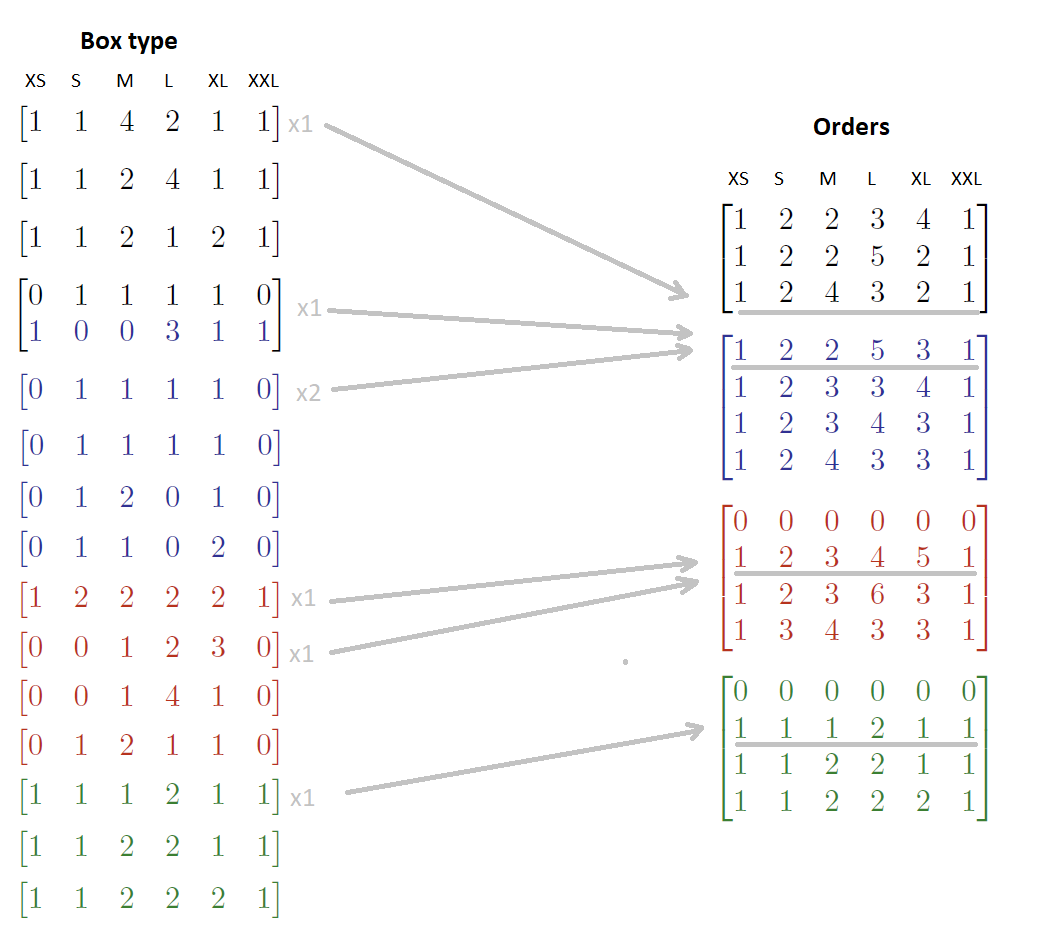
\includegraphics[width=8cm]{./figures/boxtypes.png}        \label{fig:my_label}
    \end{figure}
\end{frame}


\end{document}
